\section{Question 3}

\begin{question}
    For $f(x) = \ln x$,
\end{question}

\subsection{Part a}

\begin{question}
    Construct Lagrange interpolating polynomials of degree $n = 1,2,3$ for $f(x)$ given nodes $x_0 = 0.5$, $x_1 = 1$, $x_2 = 1.5$, and $x_3 = 2$. (Use $x_0$ and $x_1$ for $n = 1$, and add $x_2$ for $n = 2$)
\end{question}

\begin{answer}
    \begin{align}
        P_1(x) &= \tfrac{x - 1}{0.5 - 1}\cdot \ln{(0.5)}+\tfrac{x - 0.5}{1 - 0.5} \cdot \ln{(1)} = -2\ln{(0.5)}(x - 1)\\
        P_2(x) &= \tfrac{(x - 1)(x - 1.5)}{(0.5 - 1)(0.5 - 1.5)} \cdot \ln{(0.5)} + \tfrac{(x - 0.5)(x - 1.5)}{(1 - 0.5)(1 - 1.5)} \cdot \ln{(1)} + \tfrac{(x - 0.5)(x - 1)}{(1.5 - 0.5)(1.5 - 1)} \cdot \ln{(1.5)}\\
        &= 2\ln{(0.5)}(x - 1)(x - 1.5) + 2\ln{(1.5)}(x - 0.5)(x - 1)\\
        P_3(x) &= \tfrac{(x - 1)(x - 1.5)(x - 2)}{(0.5 - 1)(0.5 - 1.5)(0.5 - 2)} \cdot \ln{(0.5)} + \tfrac{(x - 0.5)(x - 1.5)(x - 2)}{(1 - 0.5)(1 - 1.5)(1 - 2)} \cdot \ln{(1)}\\
        &+ \tfrac{(x - 0.5)(x - 1)(x - 2)}{(1.5 - 0.5)(1.5 - 1)(1.5 - 2)} \cdot \ln{(1.5)} + \tfrac{(x - 0.5)(x - 1)(x - 1.5)}{(2 - 0.5)(2 - 1)(2 - 1.5)} \cdot \ln{(2)}\\
        &= - \tfrac{4\ln{(0.5)}}{3}(x - 1)(x - 1.5)(x - 2) - 4\ln{(1.5)}(x - 0.5)(x - 1)(x - 2)\\
        &+ \tfrac{4\ln{(2)}}{3}(x - 0.5)(x - 1)(x - 1.5)
    \end{align}    
\end{answer}

\subsection{Part b}

\begin{question}
    Plot $f(x)$ and all three Lagrange interpolating polynomials in \MATLAB over the interval $[0,3]$. Which does the best at approximating $f(x)$?
\end{question}

\begin{answer}
    I plot using the code below
    \begin{verbatim}
        x = linspace(0,3,100);
        P = log(x);
        P1 = 2*log(0.5)*(x-1);
        P2 = 2*log(0.5).*(x-1).*(x-1.5)+2*log(1.5).*(x-0.5).*(x-1);
        P3 = -((4*log(0.5))/3)*(x-1).*(x-1.5).*(x-2) 
        - 4*log(1.5)*(x-0.5).*(x-1).*(x-2) 
        + ((4*log(2))/3)*(x-0.5).*(x-1).*(x-1.5);
        plot(x,P,x,P1,x,P2,x,P3);
        legend({'P','P1','P2','P3'},'Location','southeast'
        ,'Orientation','horizontal');
    \end{verbatim}
    \begin{figure}[H]
        \centering
        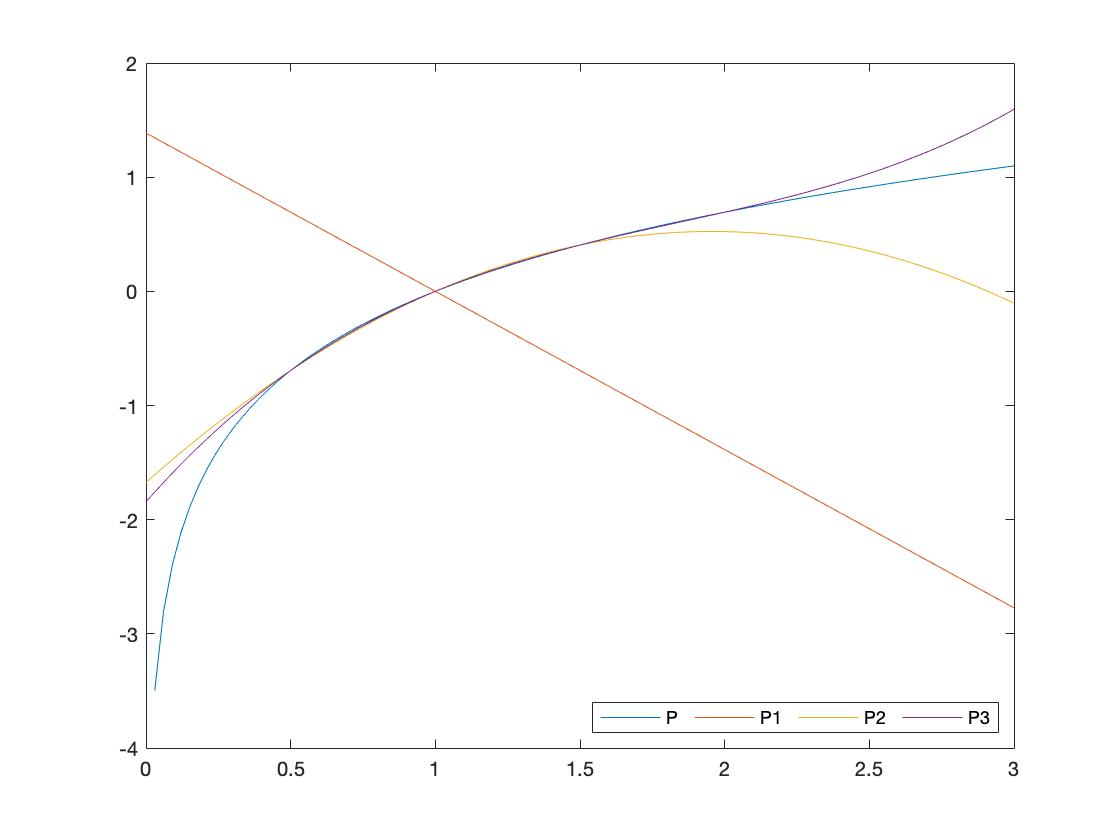
\includegraphics[width=0.9\textwidth]{Figure 5.jpg}
        \caption{\label{fig:fig5}Plot of f(x) and the Lagrange interpolating polynomials over [0,3]}
    \end{figure}
    The plot of the polynomials over the interval $[0,2]$ is shown in the Figure \ref{fig:fig5}. The third degree Lagrange interpolating polynomial does best at approximating $f(x)$, since it follows the trend of $f(x)$ and it almost overlaps with $f(x)$.
\end{answer}

\subsection{Part c}

\begin{question}
    In a new figure, plot $f(x)$ and all three Lagrange interpolating polynomials over the interval $[0,10]$. Which doest the best at approximating $f(x)$ now? What would you change (besides the interval) to make these approximations better?
\end{question}

\begin{answer}
    I plot using the following code
    \begin{verbatim}
        x = linspace(0,10,100);
        P = log(x);
        P1 = 2*log(0.5)*(x-1);
        P2 = 2*log(0.5).*(x-1).*(x-1.5)+2*log(1.5).*(x-0.5).*(x-1);
        P3 = -((4*log(0.5))/3)*(x-1).*(x-1.5).*(x-2) 
        - 4*log(1.5)*(x-0.5).*(x-1).*(x-2) 
        + ((4*log(2))/3)*(x-0.5).*(x-1).*(x-1.5);
        plot(x,P,x,P1,x,P2,x,P3);
        legend({'P','P1','P2','P3'},'Location','southeast',
        'Orientation','horizontal');
    \end{verbatim}
    \begin{figure}[H]
        \centering
        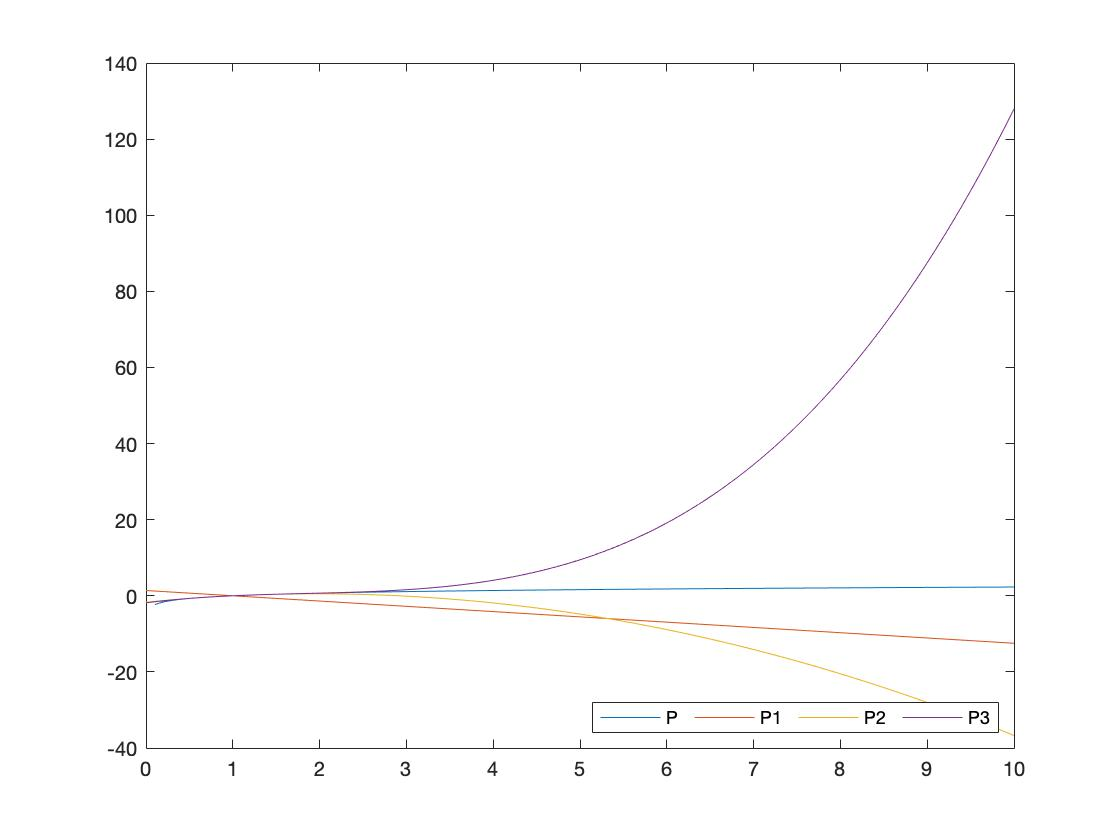
\includegraphics[width=0.9\textwidth]{Figure 6.jpg}
        \caption{\label{fig:fig6}Plot of f(x) and the Lagrange interpolating polynomials over [0,10]}
    \end{figure}
    The plot of the Lagrange interpolating polynomials over the interval $[0,10]$ is exhibited in the Figure \ref{fig:fig6}. This time, the first degree Lagrange interpolating polynomials approximate $f(x)$ the best. We can use the Newton's divided difference interpolating polynomials to make these approximations better.
\end{answer}